\chapter{Baseline urban design}

\AddToShipoutPictureBG*{%
  \AtPageUpperLeft{%
    \hspace*{18.25cm}%
    \raisebox{-3.25cm}{%
      \makebox[0pt][r]{\parbox{\textwidth}{\begin{flushright}\textit{``Scientists investigate that which already is;\\ Engineers create that which has never been.''}\\
      Albert Einstein\end{flushright}}}
}}}%

In this chapter, a baseline model is established based on the newest version of UWG for a typical district in downtown Abu Dhabi (UAE). The baseline model is validated using the measurements in 2016 for the subsequent research.

\section{Case study in Abu Dhabi}

Abu Dhabi has been developed rapidly over the past 60 years. Its climate is characterized by a very hot summer from July to September and a mild winter from December to February. The city experiences an environment with generally high temperatures and insufficient rainfall throughout the year. The K\"{o}ppen climate classification subtype for Abu Dhabi is BWh (tropical and subtropical desert climate).

This case study was conducted in District E3 (see \textbf{Figure 3-1}), which is representative of the large city blocks in downtown Abu Dhabi. The total land area of District E3 is about 193,351 m$^2$. As shown in \textbf{Figure 3-1(b)}, there is a row of high-rise residential, office, and hotel buildings on the outer borders surrounding a number of medium- and low-rise buildings in the inner part. In total, 70 buildings are considered in the baseline model, including 59 residential buildings, five office buildings, three hotels, one mosque, one school, and one hospital. In general, the buildings built in the 1990s have smaller window-to-wall ratios, while the buildings built after 2000 are mostly glazed over the fa\c{c}ade. This makes Abu Dhabi an interesting case with heterogeneous building forms located in a tropical or subtropical climate zone.

\begin{figure}
\centering
\includegraphics[width=.73\linewidth,trim=1 1 1 1,clip]{DistrictE3.pdf}
\caption{District E3 in downtown Abu Dhabi (UAE).}
\end{figure}

\begin{table}[]
\footnotesize
\begin{center}
\caption{Inputs of the UWG used in the baseline model with field data from District E3 in Abu Dhabi.}
\label{my-label}
\begin{tabular}{ll}
\toprule
Parameter                                    & Setting                 \\ \hline 
\rule{0pt}{4ex} \textit{General information} \vspace{6pt}                &                         \\
\hspace{12pt}Location                                     & Abu Dhabi               \\
\hspace{12pt}Latitude                                     & 24.490$^{\circ}$                 \\
\hspace{12pt}Longitude                                    & 54.366$^{\circ}$                 \\
\hspace{12pt}Simulation time-step                         & 300 s                   \\
\hspace{12pt}Weather data time-step                       & 3600 s                  \\
\hspace{12pt}Simulation period for validation                            & 10/01/2016 -- 10/07/2016 \\
                                             & 11/01/2016 -- 11/07/2016 \\
                                             & 12/01/2016 -- 12/07/2016 \vspace{6pt} \\
\vspace{6pt}\textit{Meteorological factors}              &                         \\
\hspace{12pt}Daytime urban boundary layer height          & 700 m                   \\
\hspace{12pt}Nighttime urban boundary layer height        & 80 m                    \\
\hspace{12pt}Reference height of the VDM                  & 150 m                   \\
\hspace{12pt}RSM temperature reference height             & 10 m                    \\
\hspace{12pt}RSM wind reference height                    & 10 m                    \\
\hspace{12pt}Circulation coefficient                      & 1.2                     \\
\hspace{12pt}UCM-UBL exchange coefficient                 & 0.3                     \\
\hspace{12pt}Heat flux threshold for daytime conditions   & 200 W m$^{-2}$               \\
\hspace{12pt}Heat flux threshold for nighttime conditions & 50 W m$^{-2}$                \\
\hspace{12pt}Minimum wind velocity                        & 0.1 m s$^{-1}$               \\
\hspace{12pt}Rural average obstacle height \vspace{6pt}               & 0.1 m                   \\
\vspace{6pt}\textit{Urban characteristics}               &                         \\
\hspace{12pt}Average building height                      & 35 m                    \\
\hspace{12pt}Fraction of waste heat into canyon           & 0.3                     \\
\hspace{12pt}Building density                             & 0.24                    \\
\hspace{12pt}Vertical-to-horizontal ratio                 & 2.2                     \\
\hspace{12pt}Urban area characteristic length             & 1000 m                  \\
\hspace{12pt}Road albedo                                  & 0.165                   \\
\hspace{12pt}Pavement thickness                           & 1.25 m                  \\
\hspace{12pt}Traffic sensible anthropogenic heat (peak)   & 19.6 W m$^{-2}$              \\
\hspace{12pt}Traffic latent anthropogenic heat (peak) \vspace{6pt}    & 2.0 W m$^{-2}$               \\
\vspace{6pt}\textit{Vegetation variables}                &                         \\
\hspace{12pt}Urban vegetation coverage                    & 0.01                    \\
\hspace{12pt}Urban tree coverage                          & 0.01                    \\
\hspace{12pt}Start month of vegetation participation      & January                 \\
\hspace{12pt}End month of vegetation participation        & December                \\
\hspace{12pt}Vegetation albedo                            & 0.25                    \\
\hspace{12pt}Latent fraction of grass                     & 0.6                     \\
\hspace{12pt}Latent fraction of tree                      & 0.7                     \\
\hspace{12pt}Rural vegetation coverage                    & 0.01                    \\
\bottomrule
\end{tabular}
\end{center}
Note: Detailed physical definition of the parameters can be found in Refs. \cite{bueno2013urban,bueno2013calculation}. In particular, Ref. \cite{bueno2013urban} illustrates the parameters in the rural station model (RSM) and urban canopy-building energy model (UC-BEM), while Ref. \cite{bueno2013calculation} illustrates the parameters in the vertical diffusion model (VDM) and urban boundary layer model (UBLM).
\end{table}


\begin{table}[]
\footnotesize
\begin{center}
\caption{Building parameters for the detailed model (DM) in the UWG.}
\label{my-label}
\makebox[\linewidth]{
\begin{tabular}{lllllll}
\toprule
Building parameter              & Residential & Hotel  & Office  & Mosque & School & Hospital \\ \hline
Total floor area (m$^2$)           & 382,086     & 99,666 & 140,886 & 2070   & 15,159 & 10,589   \\
Glazing ratio                   & 0.39        & 0.75   & 0.72    & 0.11   & 0.34   & 0.90      \\
Wall U-value (W m$^{-2}$ K$^{-1}$)        & 2.70         & 2.27   & 1.71    & 2.70    & 2.70    & 1.71     \\
Roof U-value (W m$^{-2}$ K$^{-1}$)        & 0.74        & 0.74   & 0.53    & 0.74   & 0.74   & 0.53     \\
Window U-value (W m$^{-2}$ K$^{-1}$)      & 3.88        & 2.40    & 2.40     & 3.88   & 3.88   & 2.40      \\
Window SHGC                     & 0.75        & 0.36   & 0.36    & 0.75   & 0.75   & 0.36     \\
Infiltration rate (ACH)         & 0.75        & 0.50    & 0.30     & 0.75   & 0.75   & 0.20      \\
Lighting load density (W m$^{-2}$)   & 8           & 10     & 12      & 8      & 15     & 15       \\
Equipment load density (W m$^{-2}$)  & 12          & 13     & 15      & 5      & 10     & 15       \\
Occupancy density (m$^2$ person$^{-1}$) & 25          & 10     & 10      & 10     & 8      & 15       \\
Indoor air temperature set point ($^{\circ}$C)       & 22          & 22     & 22      & 22     & 22     & 22       \\
Chiller COP                     & 2.5         & 2.5    & 2.5     & 2.5    & 2.5    & 2.5      \\
\bottomrule
\end{tabular}
}
\end{center}
Note: The values are determined based on the corresponding data taken from the local building design/energy codes provided by the Abu Dhabi Municipality (via personal contact), the on-site survey, and the prevailing engineering practices \cite{martin2015estimation,deru2011us,radhi2009evaluating,afshari2014life}.
\end{table}

The parameters used for establishing the baseline model can be categorized into four groups: meteorological factors, urban characteristics, vegetation variables, and building systems. Since detailed data collection efforts on building properties would become impractical at the urban scale, it is necessary to abstract a building stock into ``building archetypes.'' While such division is of tremendous importance for modeling reliability, the process usually remains \textit{ad hoc} based on generic assumptions. In our case study, the descriptions of the baseline model are based on careful selections of typical design and construction with corresponding data taken from the Abu Dhabi Municipality (via personal contact) and prevailing engineering practices \cite{martin2015estimation,bueno2013urban,bueno2014computationally,bueno2013calculation,deru2011us,radhi2009evaluating,afshari2014life}. A summary of the key input parameters is shown in \textbf{Tables 3.1 and 3.2}. The structural elements of the DOE reference buildings based on the Miami climate are modified according to the current building descriptions, since the climate in Miami is quite similar to that in Abu Dhabi.

\section{Model of anthropogenic heat flux}

In urban studies, anthropogenic heat flux is defined as the heat released due to human activities \cite{oke2002boundary}. According to Sailor \cite{sailor2011review}, it generally includes the heat from building operation, traffic vehicles, and human metabolism.

A methodology is proposed to evaluate the aggregated effect of building energy models on the outdoor microclimate conditions in the subsequent uncertainty/sensi-tivity analysis and model calibration. The underlying expectation is that the average building in a specific urban area is more thermally homogeneous and generic than each particular building. Two models of District E3 with different levels of detail are compared via UWG. The first model, referred to as the detailed model (DM), includes the exact information for the six building archetypes extracted from available resources. The second model, referred to as the averaged model (AM), maintains the assumptions of the building energy model but considers only one building archetype using weighted average values. The key parameters of the building geometry, energy load, and HVAC system are all set as weighted averages based on corresponding area or volume. We assume that the schedules for each building prototype cannot be averaged and thus remain unchanged. This method is adopted only if the objective is to evaluate the overall energy consumption of a neighborhood area, rather than the energy performance of a specific building. \textbf{Tables 3.2 and 3.3} summarize the parameters in DM and AM, respectively.

\begin{table}[]
\footnotesize
\begin{center}
\caption{Building parameters for the averaged model (AM) in the UWG.}
\label{my-label}
\begin{tabular}{ll}
\toprule
Building parameter                    & Weighted average \\ \hline
Glazing ratio                         & 0.48             \\
Wall U-value (W m$^{-2}$ K$^{-1}$)              & 2.5              \\
Roof U-value (W m$^{-2}$ K$^{-1}$)              & 0.7              \\
Window U-value (W m$^{-2}$ K$^{-1}$)            & 3.25             \\
Window SHGC                           & 0.58             \\
Infiltration rate (ACH)               & 0.6              \\
Lighting load density (W m$^{-2}$)         & 10               \\
Equipment load density (W m$^{-2}$)        & 13               \\
Occupancy density (m$^2$ person$^{-1}$)       & 19               \\
Indoor air temperature set point ($^{\circ}$C) & 22               \\
Chiller COP                           & 2.5              \\
\bottomrule
\end{tabular}
\end{center}
Note: The wall-, window-, and roof-related parameters are averaged based on the wall, window, and roof area, respectively. The internal heat gains are averaged based on the floor area. The infiltration level is averaged based on the building volume.
\end{table}

In the meantime, there has been a completed research project working exclusively on quantifying the traffic-related anthropogenic heat in District E3 \cite{afshari2017estimation}, since the outdoor metabolic heat is negligible and the building-related waste heat can be calculated by the UWG. The novelty of the method lies in the assumption that the air quality measurements can be a proxy for traffic intensity. In particular, the BTEX (Benzene, Toluene, Ethylbenzene, and m-, p-, o-Xylenes) concentration levels appear strongly correlated with the traffic intensity \cite{afshari2017estimation}.

The normalized diurnal profiles of the traffic intensity were derived using the BTEX concentrations measured in a downtown air quality monitoring station near District E3 during calendar year 2012. We neglect the seasonal dependence and focus on the variance on a daily basis, since the diurnal average BTEX profile is not sensitive to seasons. As shown in \textbf{Figure 3-2}, the Friday profile is quite different from the workday profile, whereas Saturdays present wide similarities with workdays. There are two peaks at 9 am and 10 pm and one minimum at 5 am in the workday diurnal profile. The Friday profile also peaks at 10 pm, while the high values persist during the nighttime. Such differences can be explained by cultural and climatic reasons. In Abu Dhabi, it is worth noting that the weekend is Friday and Saturday; Friday is the weekly Muslim holy day, a day of public worship.

\begin{figure}
\centering
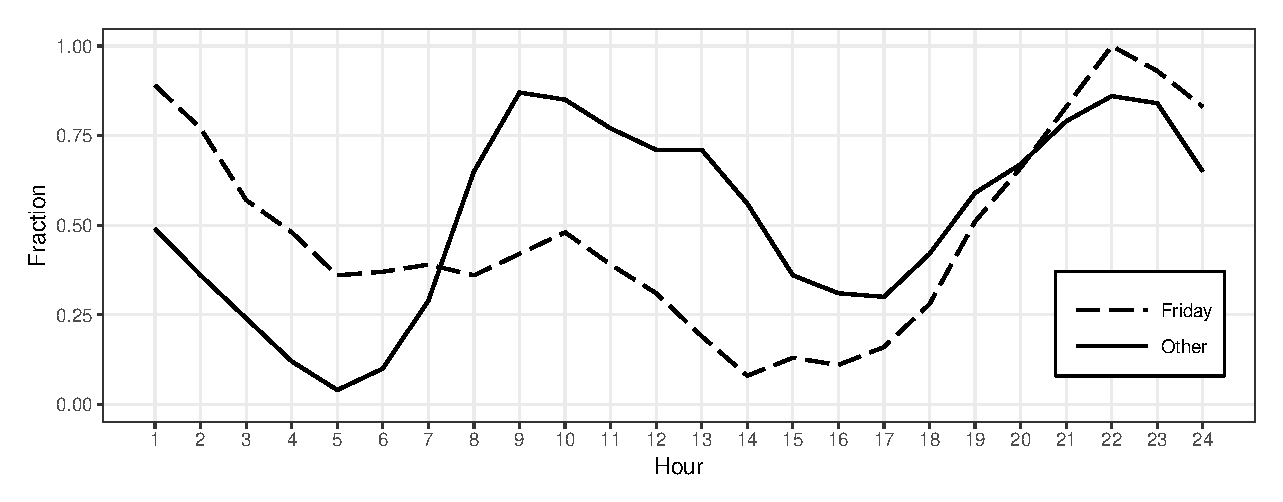
\includegraphics[width=.8\linewidth]{TrafficHeat.eps}
\caption{Normalized diurnal profile of the average traffic intensity in Abu Dhabi based on the BTEX concentration (mainly from Ref. \cite{afshari2017estimation}).}
\end{figure}

The normalized profile has been calibrated using either a bottom-up method based on high-resolution satellite images of the traffic intensity, or a top-down method based on average macro-economic and demographic variables \cite{afshari2017estimation}. Both methods have been applied and the results were quite similar. The peak traffic sensible anthropogenic heat load for the diurnal profile is 19.6 W/m$^2$, based on the full site. This is quite consistent with the result produced by Quah and Roth \cite{quah2012diurnal} in Singapore. The peak latent heat load due to motorized traffic is estimated to be 2.0 W/m$^2$.

\section{Reference and sensor data for validation}

The rural reference weather data used for the baseline model is taken from the Masdar Institute Field Station (24.436N, 54.612E), an isolated laboratory building in Masdar City. The station was built near the Abu Dhabi International Airport, 28 km from the downtown area (see \textbf{Figure 3-1(a)}). The rural station is basically surrounded by deserts connecting Abu Dhabi, Dubai, and Al Ain. Due to regular maintenance to ensure data quality, the measured data during calendar year 2016 is used for running the UWG to validate the baseline model. As shown in \textbf{Figure 3-3}, Abu Dhabi has a maximum temperature in August 2016 (about 47.3 $^{\circ}$C) and a minimum temperature in February 2016 (about 8.7 $^{\circ}$C).

\begin{figure}
\centering
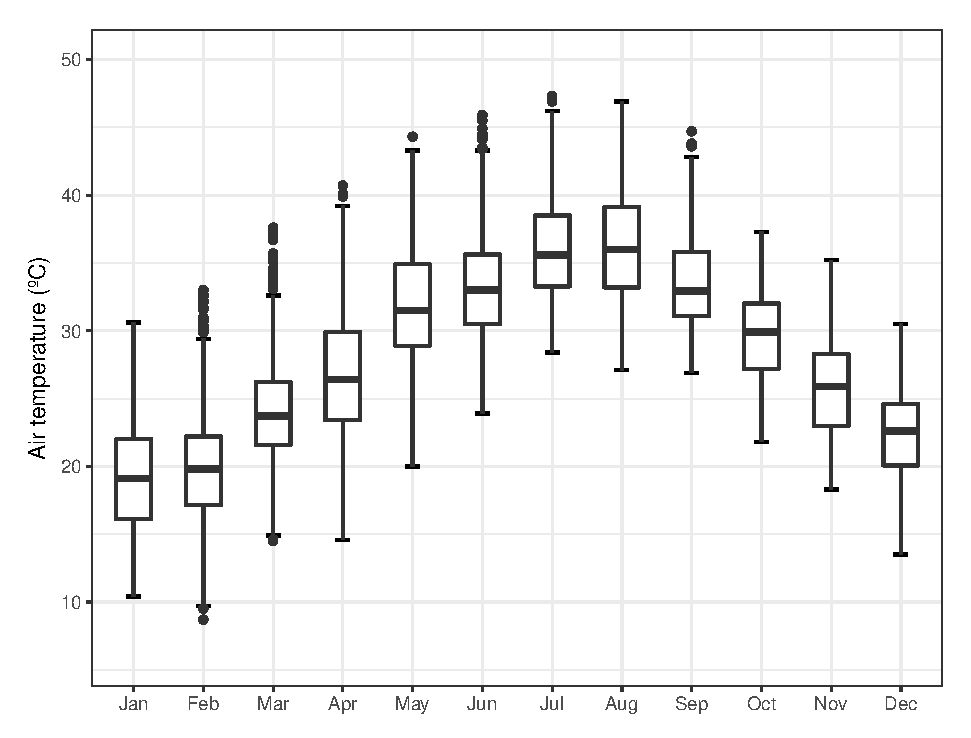
\includegraphics[width=.6\linewidth]{Weather2016.eps}
\caption{Monthly outdoor air temperature measured at the rural station in Abu Dhabi during 2016.}
\end{figure}

Temperature observations from installed urban sensors are compared with the predicted values by the UWG baseline model. In fall 2016, several arrays of sensors were attached to six lamp poles in District E3 at different sites, representing a range of land usages, morphological parameters, building operations, etc. Each sensor array consists of temperature measurements (at 3, 4, 5.5, 7, and 8.5 m), relative humidity measurements (at 3 m), and wind measurements (at 6 m, only available in four of the six stations). The sensors were inspected against each other before deployment to ensure relative accuracy of readings.

We use the data measured in 2016 from three of the calibrated sensors that present consistent performances for validating the baseline model. The corresponding locations in (latitude, longitude) of the three sensors are (24.4902$^{\circ}$, 54.3654$^{\circ}$), (24.4894$^{\circ}$, 54.3663$^{\circ}$), and (24.4907$^{\circ}$, 54.3660$^{\circ}$). In particular, the temperature observations at 8.5 m are selected for the subsequent comparison, since they are more suitable to validate the current UWG outputs for this case study (given that the average building height is 35 m).

\section{Prediction of urban outdoor air temperature}

\textbf{Figure 3-4} compares the weekly-average profiles of rural and urban outdoor air temperature calculated by the model from October to December 2016. The diurnal pattern of UHI is characterized by a slightly cooler temperature in the urban area than in the rural area during the late morning, and a relatively warmer temperature from the afternoon to the early morning the next day. The urban-rural temperature differences are more intense in the early morning. This is quite consistent with the results from previous studies \cite{bueno2013urban,bueno2014computationally,oke2002boundary}. Generally speaking, due to the aggregate effect of the whole city, the UHI cannot be neglected in Abu Dhabi for the assessment of either thermal comfort or energy consumption.

\begin{figure}
\centering
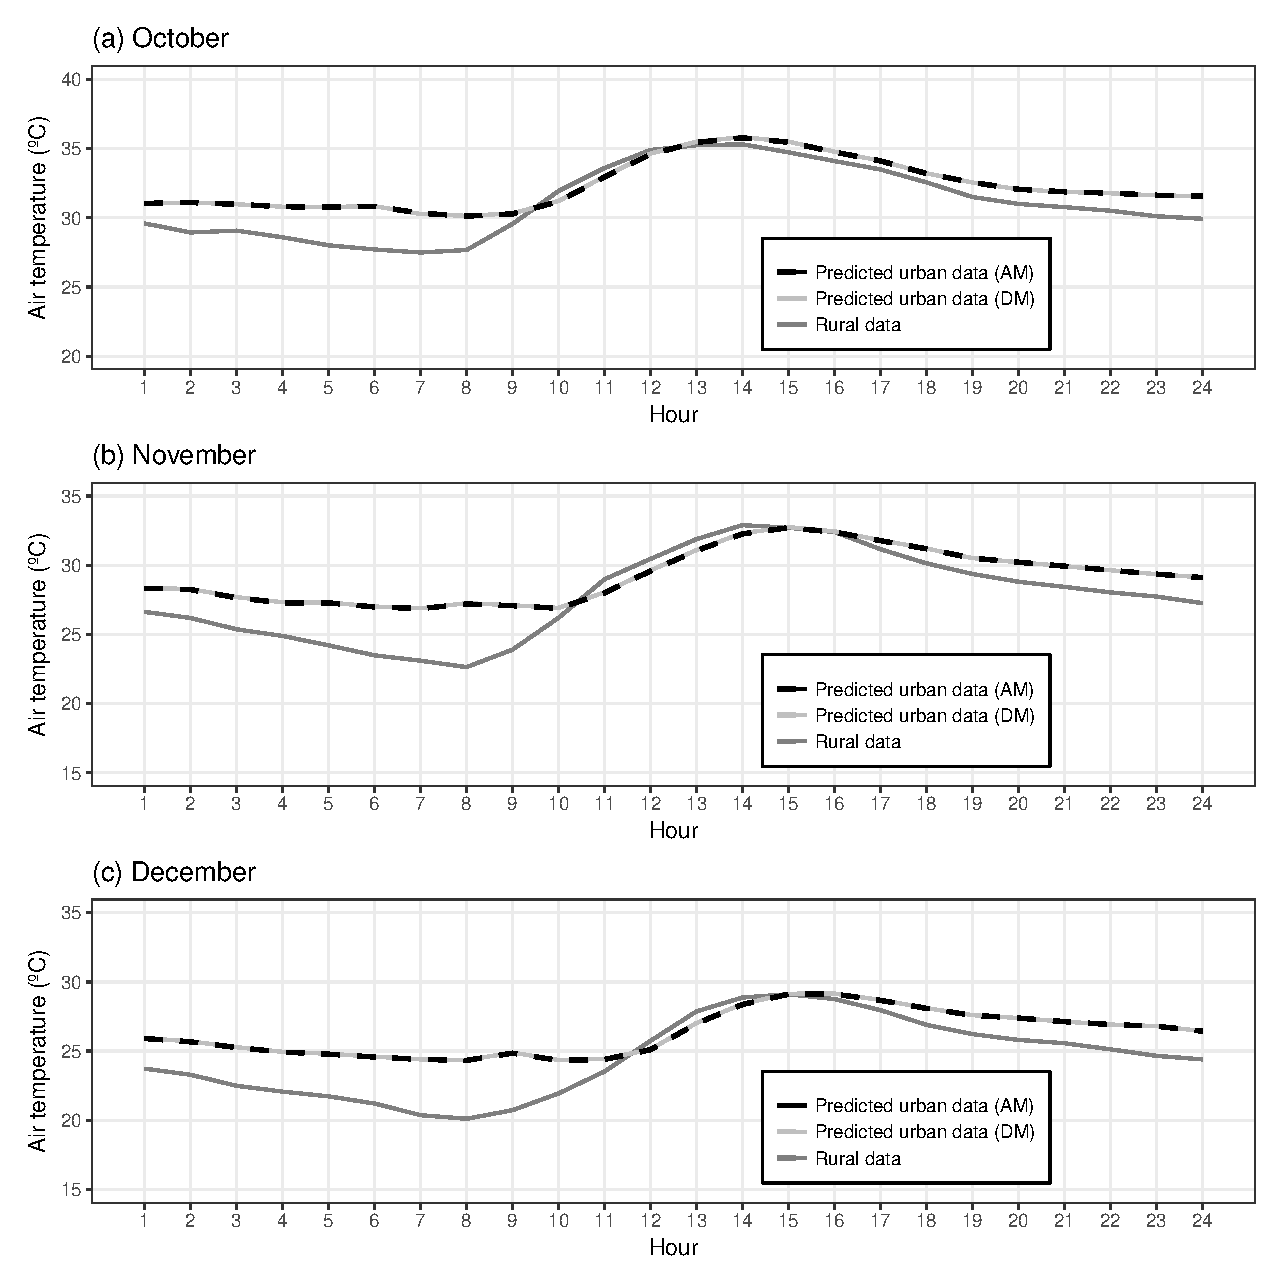
\includegraphics[width=.8\linewidth]{Figure3-4.eps}
\caption{Weekly-average diurnal profiles of the rural and urban outdoor air temperature: (a) Data between October 1 and 7, 2016; (b) Data between November 1 and 7, 2016; (c) Data between December 1 and 7, 2016.}
\end{figure}

We can also see that the DM and AM present almost the same profile of the urban outdoor air temperature. The differences in the diurnal pattern, computed as the root-mean-square error (RMSE) between the DM and AM, are all about 0.03 $^{\circ}$C from October to December. On the other hand, the difference in urban electricity use between the DM and AM can be observed to some extent in \textbf{Figure 3-5}, especially during the daytime. The corresponding diurnal differences, computed as the RMSE between the DM and AM, are respectively about 0.52, 0.59, and 0.64 MWh in October, November, and December. Usually there are more cooling demands during the daytime than during the nighttime for Abu Dhabi, resulting in more significant impacts of building-related parameters on the urban energy consumption. Nevertheless, the differences are not very high given the state of the art of urban energy modeling. This justifies the application of AM in the UWG to assess the aggregated effect of building energy models on the outdoor microclimate conditions in the subsequent uncertainty/sensitivity analysis and model calibration.

\begin{figure}
\centering
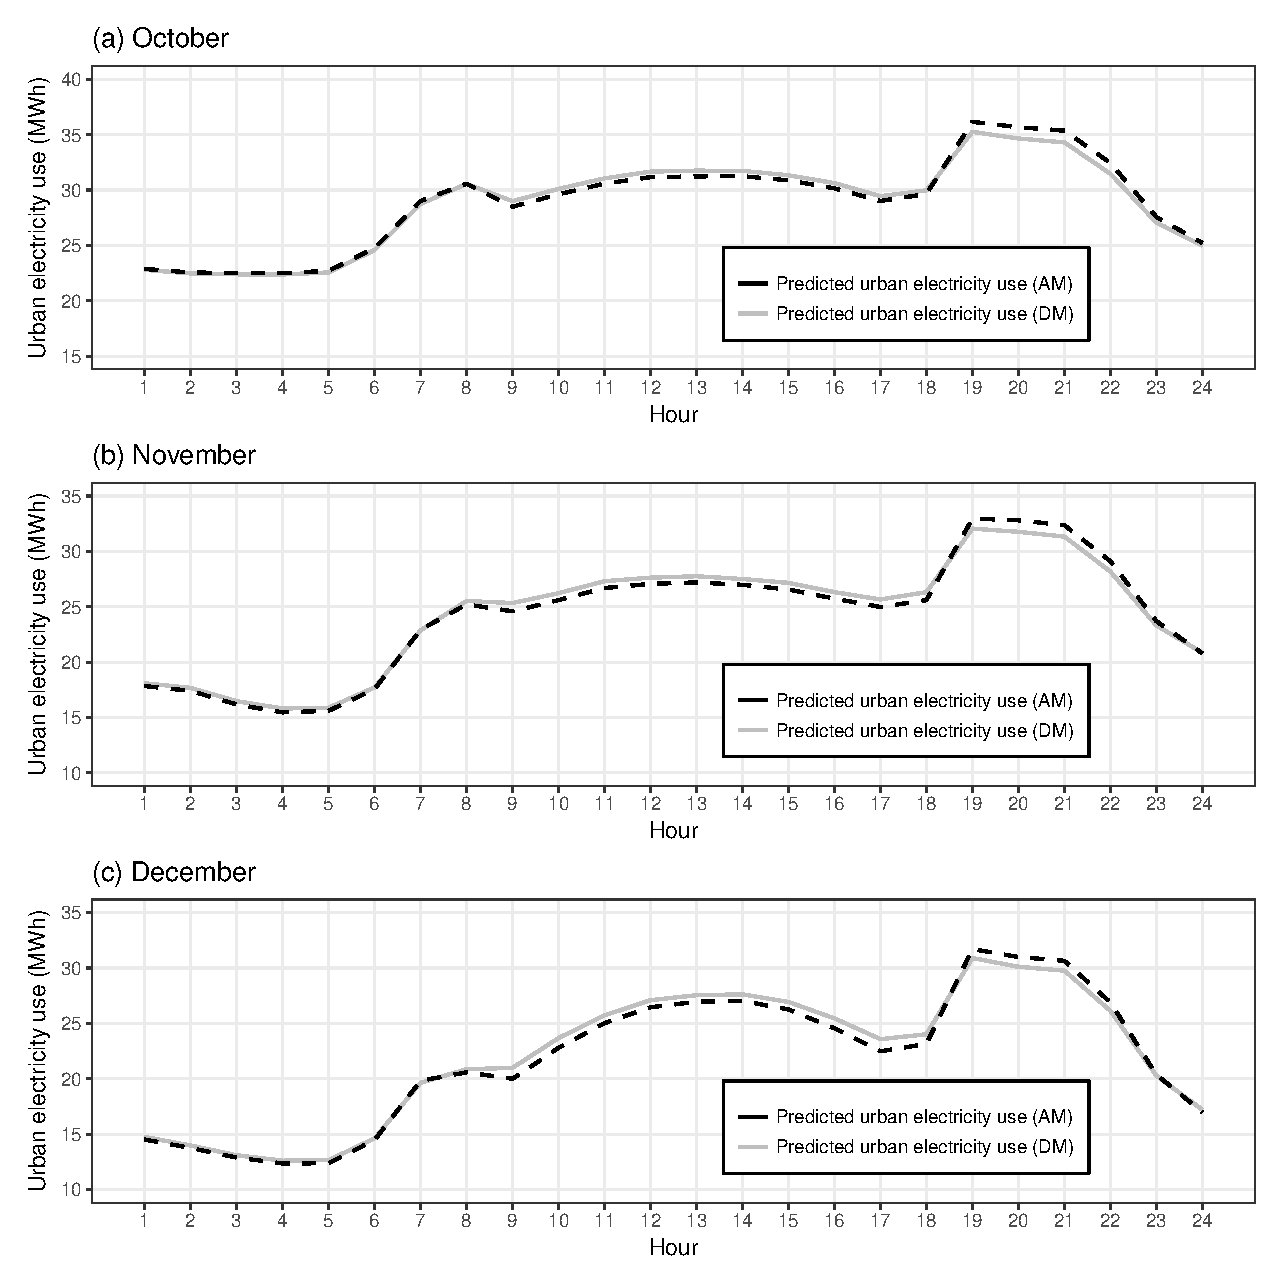
\includegraphics[width=.8\linewidth]{Figure3-5.eps}
\caption{Weekly-average diurnal profiles of the predicted urban electricity use: (a) Data between October 1 and 7, 2016; (b) Data between November 1 and 7, 2016; (c) Data between December 1 and 7, 2016.}
\end{figure}

The capacity of the UWG baseline model with the averaged building energy models to predict the urban outdoor air temperature is evaluated against the observations from October to December 2016, as shown in \textbf{Figure 3-6}. To properly describe the air temperature in the whole area of District E3 and to account for the sensor measurement uncertainty, we considered the average and standard deviation of the three sensors. \textbf{Figure 3-6} illustrates that the UWG tends to either over-predict or under-estimate the urban air temperature to some extent in the daytime. In general, the prediction performance is relatively better during the nighttime than during the daytime. Although validation of the electricity use prediction has not been performed -- due to our current inability to access such data -- we expect to obtain the corresponding meter data and will include such validation in the future. Still, considering the complexity of urban systems, the UWG can roughly capture the UHI pattern and produce some plausible values regarding the urban microclimate condition.

\begin{figure}
\centering
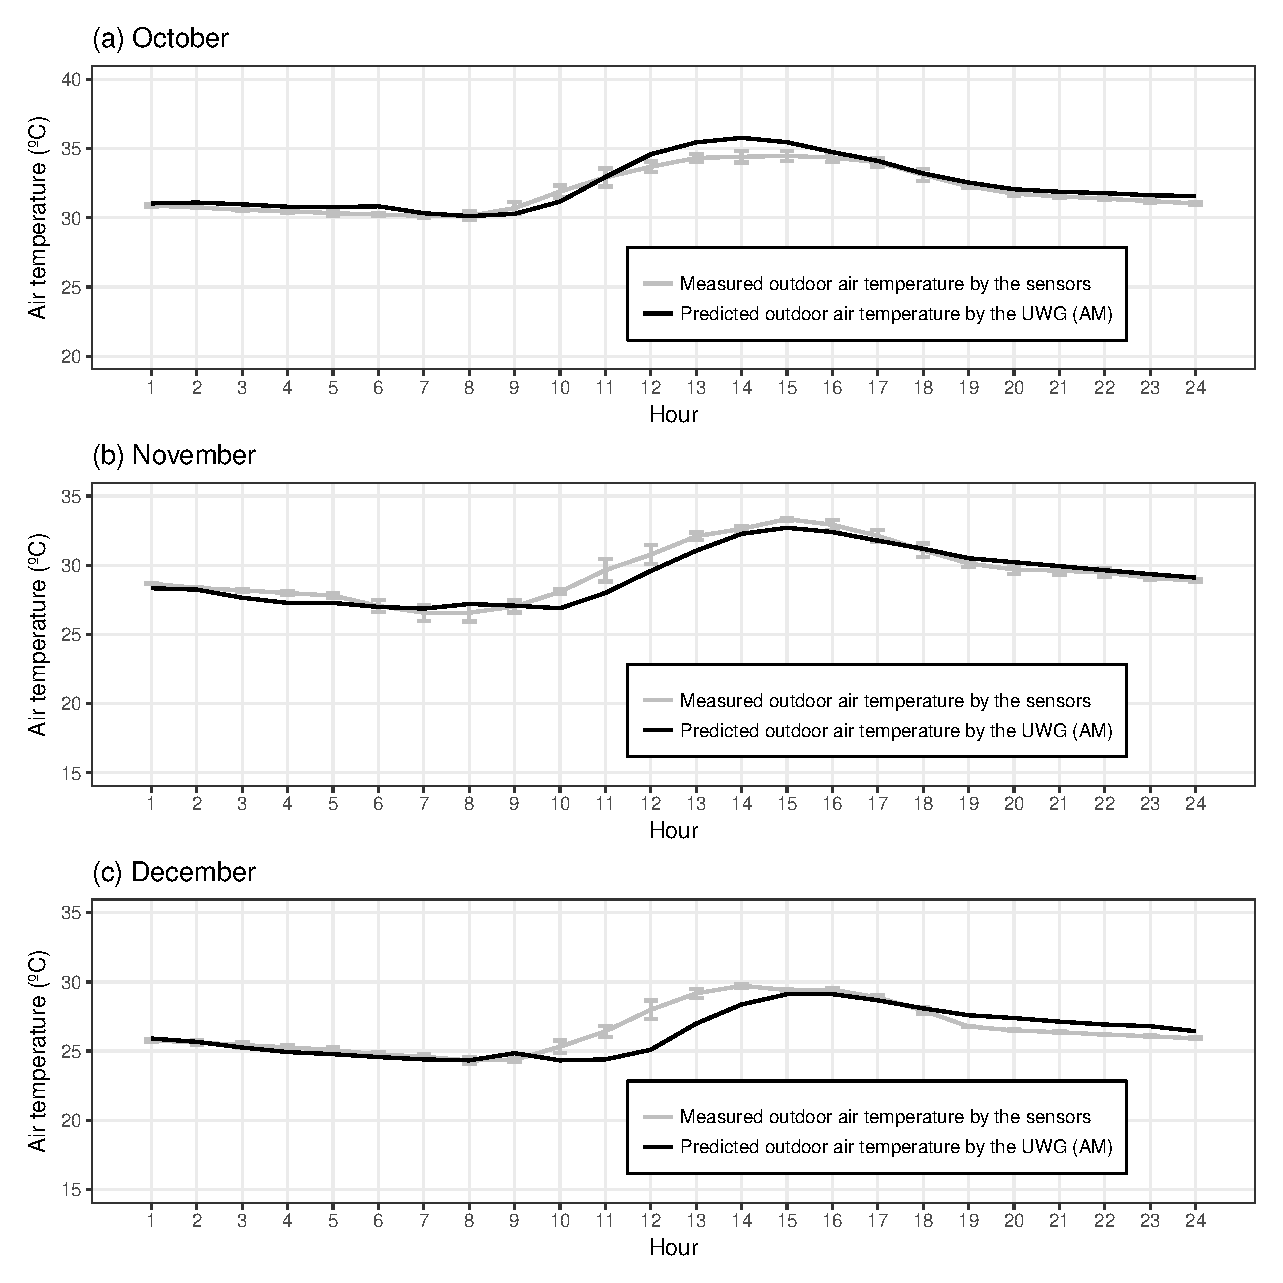
\includegraphics[width=.8\linewidth]{Figure3-6.eps}
\caption{Weekly-average diurnal profiles of the measured and predicted urban outdoor air temperature: (a) Data between October 1 and 7, 2016; (b) Data between November 1 and 7, 2016; (c) Data between December 1 and 7, 2016. The error bar represents the standard deviation of the measured urban outdoor air temperature from different sensors.}
\end{figure}
